\subsection{Data Storage and Privacy Requirements}
The MASVS defines sensitive data that concerns to both user credentials and any further data considered senstive in the following context:

\begin{itemize}
    \item Personally identifiable information (PII) that can be used for identify theft including social security numbers, credit card numbers, bank account numbers, health information.
    \item Highly sensitive data that would lead to reputational harm and/or finanical costs if compromised including contractual information, information cover by non-disclosure agreements, management information
    \item Any data that must be protected by law or for compliance reasons
\end{itemize}

Table \ref{tab:data-storage-and-privacy-requirements} describes the security requirements related to data storage and privacy.

\begin{table}
    \centering
    \caption{Data Storage and Privacy Requirements}
    \label{tab:data-storage-and-privacy-requirements}
    \begin{tabulary}{1.0\textwidth}{|L|L|}
        \hline
        \textbf{Requirement} & \textbf{Description} \\
        \hline
        Local Storage for sensitve data & System credential storage facilities need to be used to store sensitive data, such as PII, user credentials or cryptographic keys \\
        \hline
        Logs for sensitive data & Non sensitive data is written to application logs \\
        \hline
        Sensitive data in the keyboard cache & The keyboard cache is disabled on text inputs that process sensitive data \\
        \hline
        Determining whether sensitive data is exposed via ipc mechanisms & No sensitive data is exposed via IPC mechanisms \\
        \hline
        Sensitive data disclosure through the user interface & No sensitive data, such as passwords or pins, is exposed through the user interface \\
        \hline
    \end{tabulary}
\end{table}

\subsection{Authentication and Session Management}
Logging users in and managing sessions is an essential part of CheFeed. The objective of this security control is to define fundamental requirements on how user accounts and sessions are to be managed. The requirements are described in Table \ref{tab:auth-and-sessions}. 

\begin{table}
    \centering
    \caption{Authentication and Session Management Requirements}
    \label{tab:auth-and-sessions}
    \begin{tabulary}{1.0\textwidth}{|L|L|}
        \hline
        \textbf{Requirement} & \textbf{Description} \\ 
        \hline
        Verifying appropriate authentication & If the app provides users access to a remote service, some form of authentication, such as username/password authentication, is performed at the remote endpoint \\
        \hline
        User logout & The remote endpoint terminates the existing session when the user logs out \\
        \hline
        Best practices for passwords & A password policy exists and is enforced at the remote endpoint \\
        \hline
        Session timeout & Sessions are invalidated at the remote endpoint after a predefined period of inactivity and access tokens expire \\
        \hline
        Authorization models & Authorization models should be defined and enforced at the remote endpoint \\
        \hline
    \end{tabulary}
\end{table}

\subsubsection{Verifying Appropriate Authentication}
The backend must impose authorization checks from the mobile client to mitigate authentication bypass vulnerabilities. The overall authentication flow is illustrated in Figure \ref{fig:auth-flow}. When the user credentials are accepted by the endpoint, the server returns with a response that carries an access token in the header which the client must use to persist authentication and send when requesting protected resources.

\begin{figure}
    \centering
    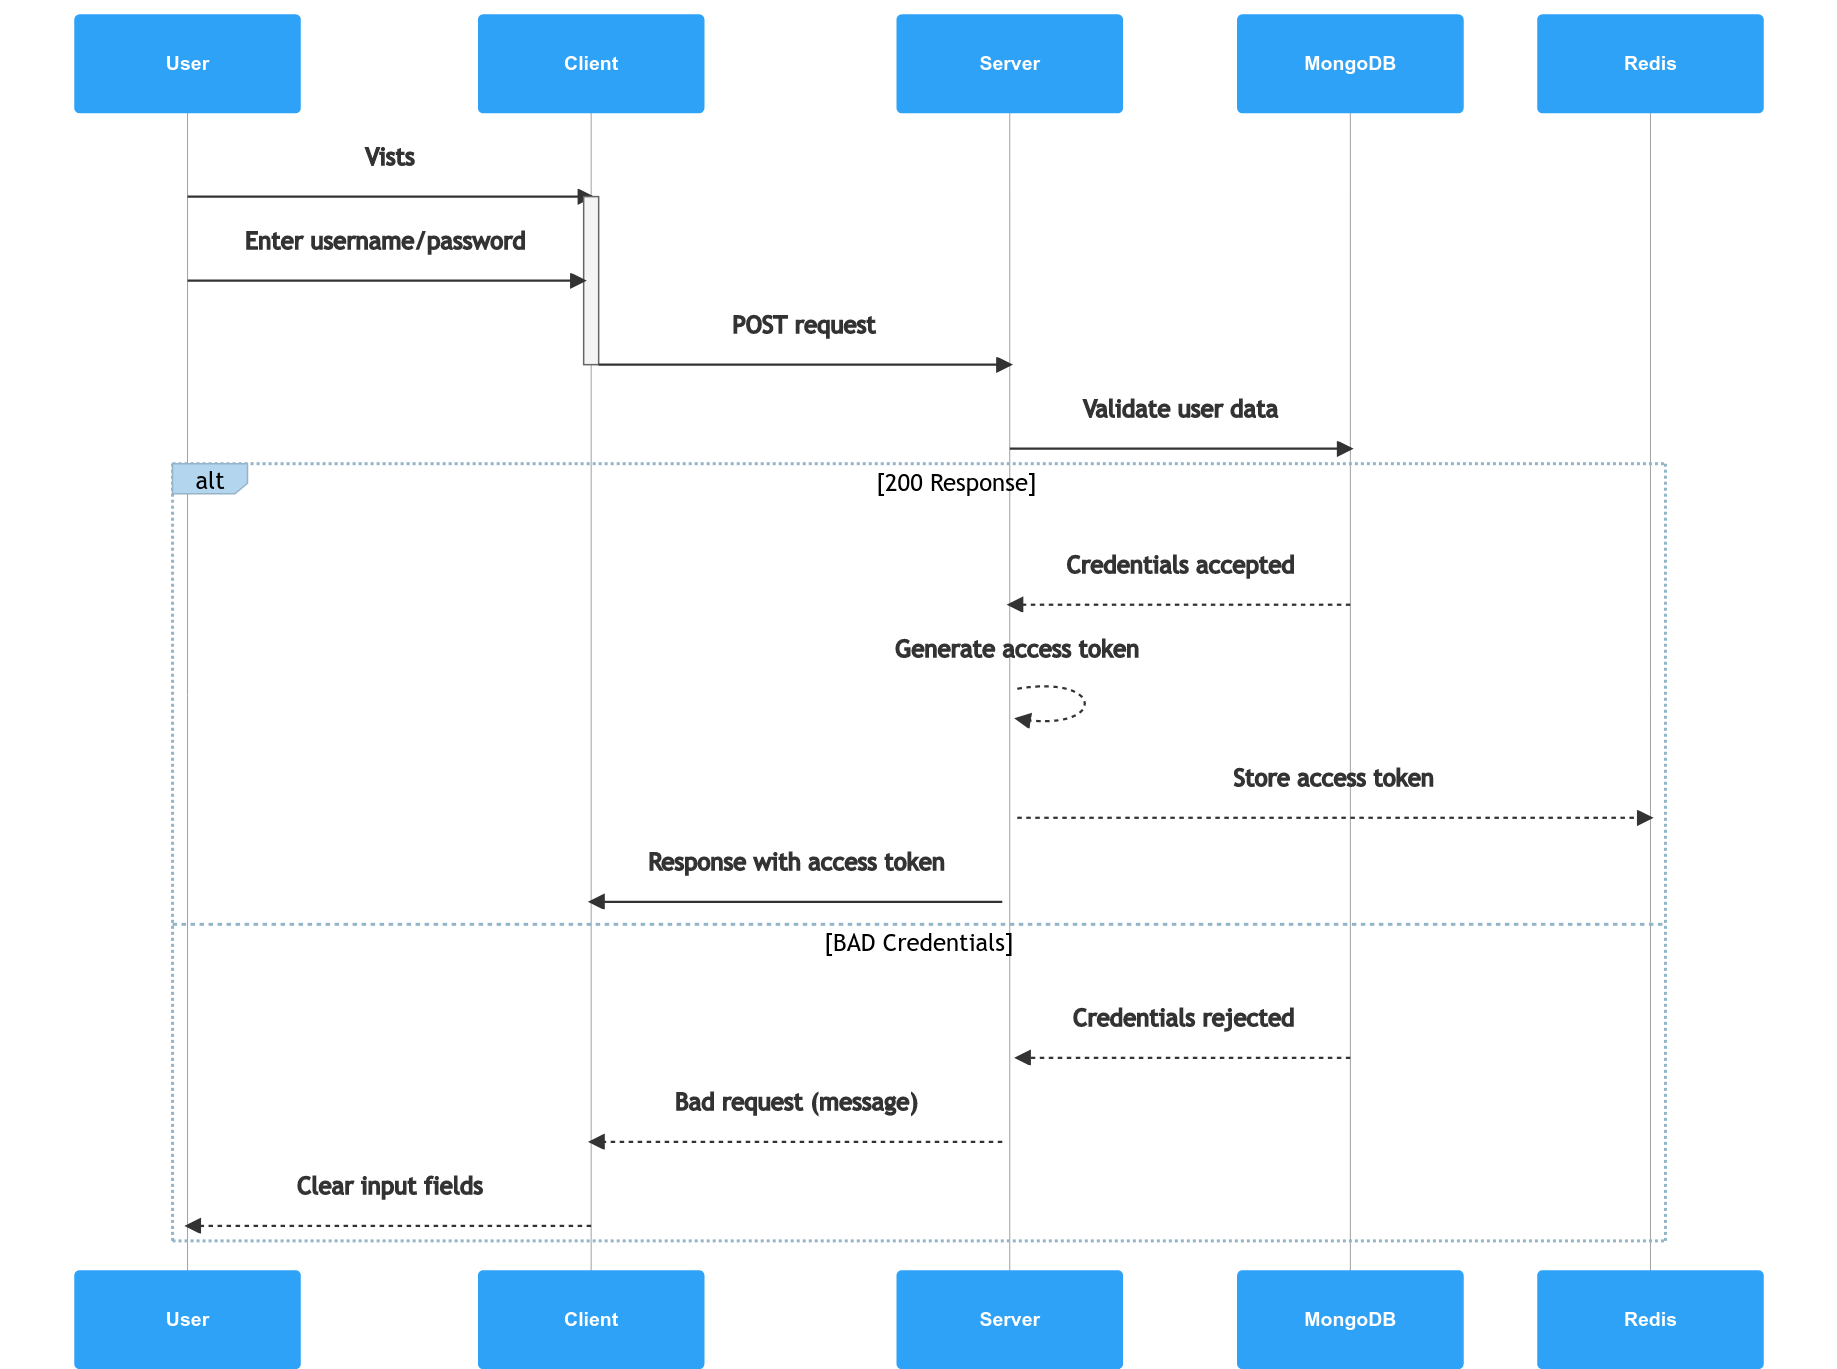
\includegraphics[width=\textwidth]{../../img/chapter-4/auth-flow.png}
    \caption{Authentication Flow}
    \label{fig:auth-flow}
\end{figure}

\subsubsection{User Logout}
When the user request to end the user session, the server must ensure the access token is invadeted from the server. The client has to ensure the token is terminated as well. Figure \ref{fig:logout-seq} illustrates the overall logout sequence.

\begin{figure}
    \centering
    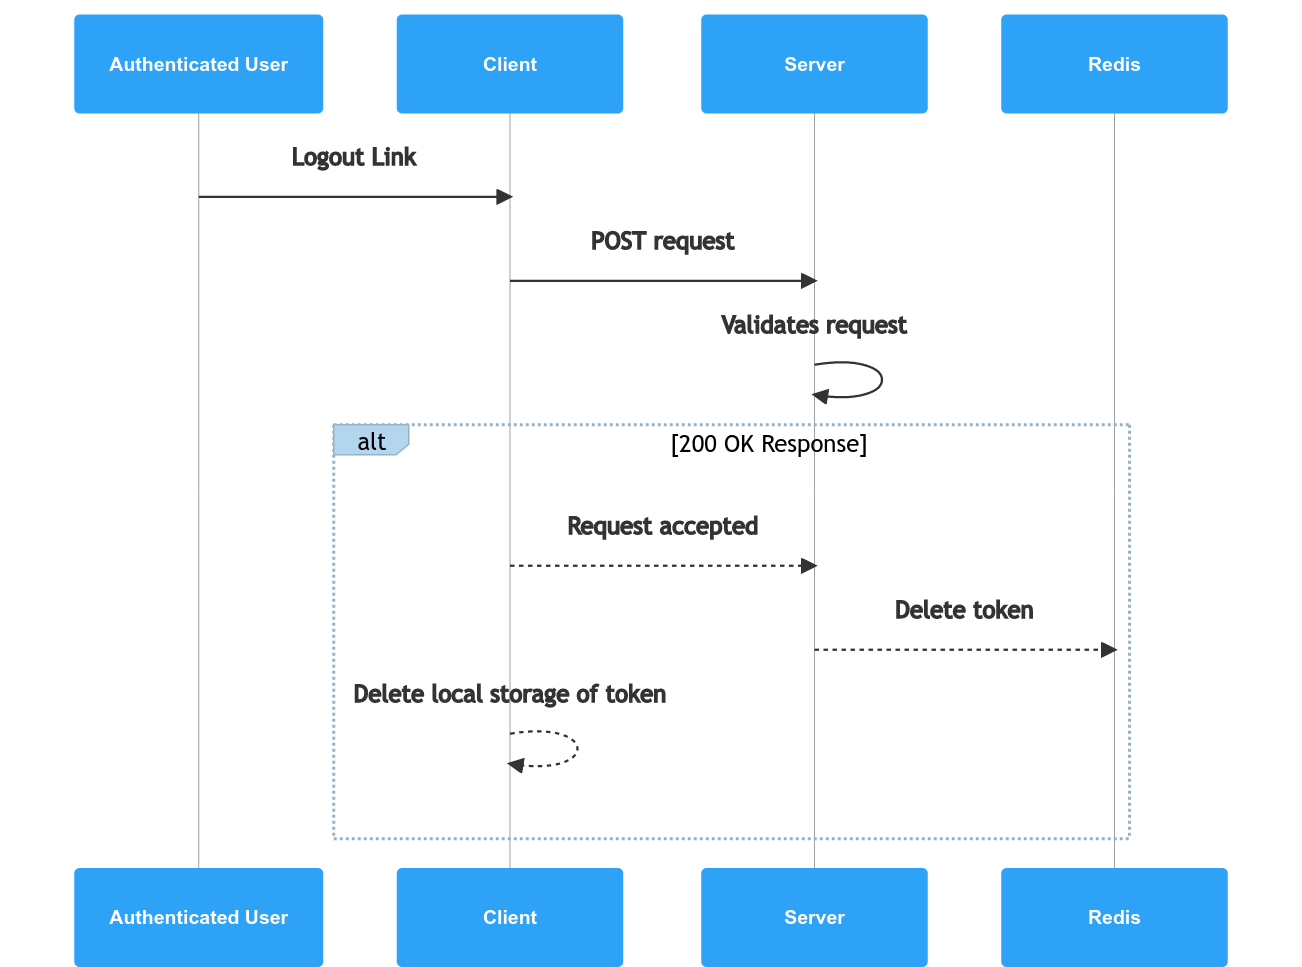
\includegraphics[width=\textwidth]{../../img/chapter-4/logout-sequence.png}
    \caption{Logout sequence}
    \label{fig:logout-seq}
\end{figure}

\subsubsection{Best Practices for Passwords}
A strong password policy ensures that manual or automated password attacks are difficult or impossible. Ensure the following attributes are met for password validation:

\begin{itemize}
    \item Ensure passwords are greater than 8 characters
    \item Passwords should not be silently truncated
    \item All characters should be allowed including Unicode and whitespace
\end{itemize}

\subsubsection{Session timeout}
Sessions must expire after a set time period. The longer a session is active, the more time an attacker is given to hijack a valid session ID and reuse it.

\subsubsection{Authorization Models}
Table \ref{tab:critical-endpoints} describes the endpoints that must enforce authorization checks. The user must be authenticated and have the appropriate authorization in place in order to make requests from these resources. Figure \ref{fig:authorization-flow} illustrates how authorizated is granted or denied. As was illustrated in Figure \ref{fig:auth-flow}, the client is given a randomly generated token from the server that grants access to the protected resources. With the bearer in the request header, the user can be granted permissions.

\begin{table}
    \caption{Critical endpoints}
    \label{tab:critical-endpoints}
    \begin{tabulary}{1.0\textwidth}{|L|L|L|}
        \hline
        \textbf{Method} & \textbf{Endpoint} & \textbf{Description} \\
        \hline
        POST & \textit{/auth/logout} & Terminates session \\
        \hline
        GET & \textit{/users/me} & Get the current user \\
        \hline
        PUT & \textit{/users/me} & Update the current user \\
        \hline
        DELETE & \textit{/users/{id}} & Delete a user by id \\
        \hline
        POST & \textit{/api/v1/recipes/new} & Create new recipe \\
        \hline
        PUT & \textit{/api/v1/recipes/{id}} & Update existing recipe with given id \\
        \hline
        DELETE & \textit{/api/v1/recipes/{id}} & Delete existing recipe with given id \\
        \hline
        POST & \textit{/api/v1/ingredients/new} & Create new ingredient \\
        \hline
        POST & \textit{/api/v1/reviews/id} & Create new review for a recipe \\
        \hline
    \end{tabulary}
\end{table}


\begin{figure}[!b]
    \centering
    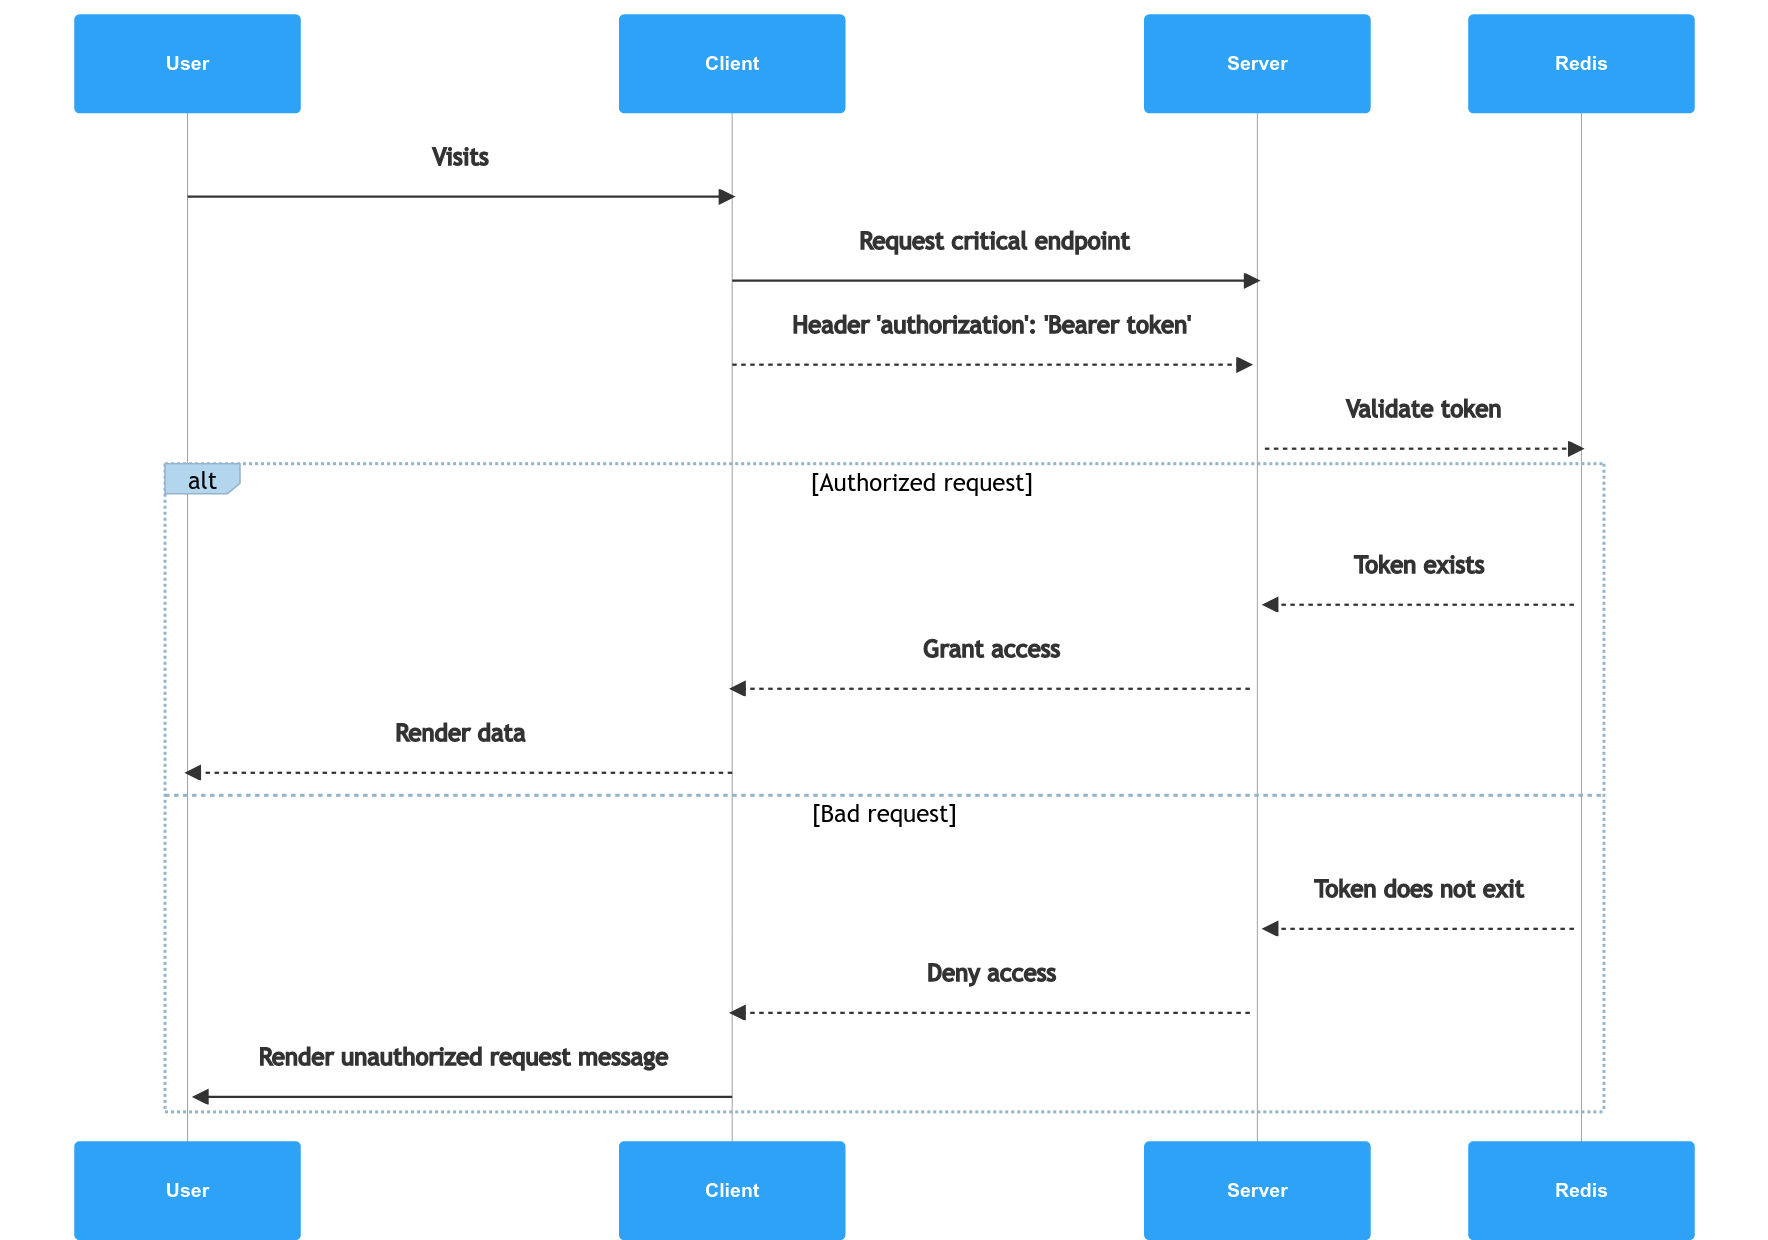
\includegraphics[width=\textwidth]{../../img/chapter-4/authorized.png}
    \caption{Authorization flow}
    \label{fig:authorization-flow}
\end{figure}

